% Frugal AI seminar, project 1: a wiki over a PDF (FrugalAI/code/quantum-wiki). Procedure and theory only, no results.
% CheatSheet-safe: no floats.

\section[PDF Wiki]{Project: A Wiki Over a PDF}

%%%%%%%%%%%%%%%%%%%%%%%%%%%%%%%%%%%%%%%%%%%%%%%%%%%
\begin{frame}[fragile]\frametitle{}
\begin{center}
{\Large Project: A Wiki Over a PDF}

\medskip
{\small (Question answering with page citations, using only small local models)}
\end{center}
\end{frame}

%%%%%%%%%%%%%%%%%%%%%%%%%%%%%%%%%%%%%%%%%%%%%%%%%%%
\begin{frame}[fragile]\frametitle{Why Plain Retrieval Is Not Enough}
\begin{itemize}
\item The usual recipe: cut the PDF text into fixed windows, embed them, retrieve the top few, let the model answer.
\item Some answers are not inside any window. In a course catalogue, ``mandatory'' or ``optional'' can live in the spanning header rows of a table, not in a column.
\item Some answers are spread over many places: ``which courses mention a topic?'' needs a join over all courses, and top-k retrieval cannot join.
\item Bullet hierarchy (topic, subtopic, sub-subtopic) is often only visible as indentation, and the same bullet glyph may be reused at deeper levels.
\item Idea: recover the structure first, then answer exact questions from the structure and keep the model for language.
\end{itemize}
{\tiny (Ref: FrugalAI code/quantum-wiki)}
\end{frame}

%%%%%%%%%%%%%%%%%%%%%%%%%%%%%%%%%%%%%%%%%%%%%%%%%%%
\begin{frame}[fragile]\frametitle{Procedure: Parse, Structure, Route}
\begin{center}
\adjustbox{max width=0.97\linewidth, max totalheight=0.26\textheight}{%
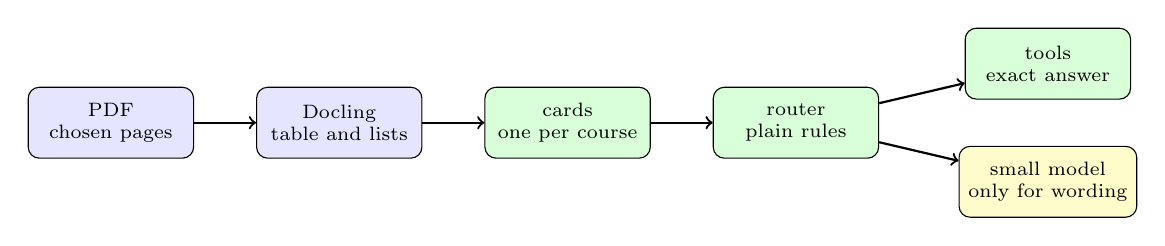
\begin{tikzpicture}
\tikzstyle{b}=[draw, rounded corners, align=center, minimum height=0.9cm, minimum width=2.1cm, font=\scriptsize]
\node[b, fill=blue!10] (p) at (0,0) {PDF\\chosen pages};
\node[b, fill=blue!10] (d) at (2.9,0) {Docling\\table and lists};
\node[b, fill=green!15] (c) at (5.8,0) {cards\\one per course};
\node[b, fill=green!15] (r) at (8.7,0) {router\\plain rules};
\node[b, fill=green!15] (t) at (11.9,0.75) {tools\\exact answer};
\node[b, fill=yellow!20] (m) at (11.9,-0.75) {small model\\only for wording};
\draw[->, thick] (p) -- (d);
\draw[->, thick] (d) -- (c);
\draw[->, thick] (c) -- (r);
\draw[->, thick] (r) -- (t);
\draw[->, thick] (r) -- (m);
\end{tikzpicture}}
\end{center}
\begin{itemize}
\item Parse once with Docling and keep the lossless document: text, tables with their spans, and the position of every list item. Cache it, do not re-parse per question.
\item Read the table's spanning rows (cells that repeat across columns) as group headers. Read list levels from indentation, not from the bullet glyph.
\item Build one ``card'' per course: status, credits, topic tree, outcomes, references, page numbers.
\end{itemize}
{\tiny (Ref: Docling; FrugalAI code/quantum-wiki)}
\end{frame}

%%%%%%%%%%%%%%%%%%%%%%%%%%%%%%%%%%%%%%%%%%%%%%%%%%%
\begin{frame}[fragile]\frametitle{Implementation: Chunks, Embeddings, Retrievers}
\begin{itemize}
\item Chunks come from the cards, one per module. Each chunk starts with a header line (course code, title, section) so it is understandable alone, and carries its page numbers.
\item Embeddings: LangChain \texttt{OpenAIEmbeddings} pointed at a local OpenAI-compatible server (LM Studio) running a small embedding model. Cache every vector on disk, and add the task prefixes the model expects.
\item Retrievers: dense search in an in-memory vector store, BM25 (\texttt{rank-bm25}), and a reciprocal-rank fusion of the two. Compare them; do not assume the hybrid wins.
\item Documents and retrievers are LangChain objects; the cards and tools are plain Python.
\item Docling is called directly and its output wrapped as LangChain documents, so the shared environment does not need the extra loader package.
\end{itemize}
{\tiny (Ref: LangChain 1.x; LM Studio local server; FrugalAI code/quantum-wiki)}
\end{frame}

%%%%%%%%%%%%%%%%%%%%%%%%%%%%%%%%%%%%%%%%%%%%%%%%%%%
\begin{frame}[fragile]\frametitle{Implementation: Tools First, Model Second, Then Check}
\begin{itemize}
\item A rule-based router sends each question to a tool: status of a course, a list by status, credits and titles, lecture counts, ``which courses mention X'', references, a course's topic tree. No rule fires: retrieval fallback.
\item Tools return an exact answer when the structure holds it, so no model call is needed. The model reads a course's own text only for open topic questions.
\item Check in plain code: every course code and every proper name in a model answer must occur in the evidence; otherwise retry once with a stricter prompt, then refuse.
\item If a tool finds nothing, say ``the syllabus does not say''. Never let the model fill the gap.
\item Evaluate with a gold question set (answers and pages), a second set of reworded questions kept apart, and the plain baselines on the same questions.
\end{itemize}
{\tiny (Ref: FrugalAI code/quantum-wiki)}
\end{frame}
